% Created 2025-01-13 Mon 21:55
% Intended LaTeX compiler: pdflatex
\documentclass[presentation]{beamer}
\usepackage[utf8]{inputenc}
\usepackage[T1]{fontenc}
\usepackage{graphicx}
\usepackage{longtable}
\usepackage{wrapfig}
\usepackage{rotating}
\usepackage[normalem]{ulem}
\usepackage{amsmath}
\usepackage{amssymb}
\usepackage{capt-of}
\usepackage{hyperref}
\nocite{*}
\usepackage[T1]{fontenc}
\usepackage[utf8]{inputenc}
\usepackage[spanish]{babel}
\usepackage[backend=biber, style=apa]{biblatex}
\addbibresource{/home/martincusme/repoArqui/bibliography.bib}
\usetheme{default}
\usecolortheme{}
\usefonttheme{}
\useinnertheme{}
\useoutertheme{}
\author{Lenin G. Falconí, Richard Dawkins, Jean LeCunn}
\date{}
\title{S9-Memoria-del-Sistema}

\hypersetup{
 pdfauthor={Lenin G. Falconí, Richard Dawkins, Jean LeCunn},
 pdftitle={S9-Memoria-del-Sistema},
 pdfkeywords={},
 pdfsubject={},
 pdfcreator={Emacs 27.1 (Org mode 9.3)}, 
 pdflang={Spanish}}
\begin{document}

\maketitle
\begin{frame}{Outline}
\tableofcontents
\end{frame}



\section{Indicaciones}
\label{sec:orga4b06de}
\begin{frame}[allowframebreaks]{Indicaciones}
\end{frame}
\begin{frame}[label={sec:orgbe6d252}]{Diseño de las Diapositivas}
\begin{itemize}
\item Para diseñar sus diapositivas puede consultar cualquiera de las
presentaciones .ORG desarrolladas por el profesor así como al
archivo \href{https://github.com/LeninGF/EPN-Lectures/blob/main/iccd332ArqComp-2024-B/Tutoriales/Beamer-Emacs/tutorialBeamer.org}{tutorialBeamer.org} en el repositorio de \href{https://github.com/LeninGF/EPN-Lectures/blob/main/iccd332ArqComp-2024-B/Tutoriales/Beamer-Emacs/tutorialBeamer.org}{GitHub} de la clase.
\item Recuerde que los archivos .ORG son archivos de texto así que los
puede copiar y sustituir por su texto propio.
\end{itemize}
\end{frame}
\begin{frame}[label={sec:orga653d3f}]{Sobre este Documento}
\begin{itemize}
\item Este documento tiene la propuesta de temas a tratar y desarrollar
por los estudiantes.
\item Se ha de utilizar como base la bibliografía recomendada, pero puede
consultar bibliografía adicional.
\end{itemize}
\end{frame}
\section{Memoria Cache (E2, 11, 162)}
\label{sec:org15c2465}
\begin{frame}[label={sec:org9c20f6a}]{Principios Básicos de las Memorias Caché (E2,11,163)(E2,7,133)}
\alert{\alert{\alert{¿Para que sirve?}}} 


El objetivo principal de la memoria caché es mejorar la velocidad de acceso a los datos almacenados, combinando el acceso rápido a datos de una memoria más cara y de alta velocidad (memoria caché) con el almacenamiento más lento pero de mayor capacidad de la memoria principal.


\alert{\alert{\alert{Funcionamiento}}}


\begin{itemize}
\item La CPU transfiere palabras o bloques entre la caché y la memoria principal. La caché actúa como intermediaria rápida entre la CPU y la memoria principal, almacenando temporalmente datos que la CPU necesita frecuentemente.
\end{itemize}
\end{frame}


\begin{frame}[label={sec:org8717944}]{Principios Básicos de las Memorias Caché (E2,11,163)(E2,7,133)}
\begin{itemize}
\item En el modelo simple de caché (como muestra la Figura 5.1a), la CPU realiza transferencias rápidas a la caché y transferencias más lentas a la memoria principal.
\end{itemize}

\begin{center}
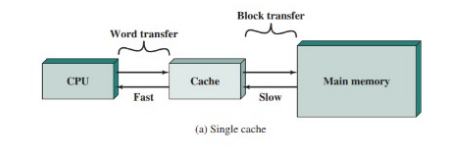
\includegraphics[width=.9\linewidth]{./Imagenes/captura1.png}
\end{center}
\end{frame}

\begin{frame}[label={sec:orgf82c844}]{Principios Básicos de las Memorias Caché (E2,11,163)(E2,7,133)}
Niveles de Caché: Se organizan en varios niveles (L1, L2, L3). A medida que se avanza en los niveles, la velocidad disminuye, pero la capacidad aumenta.

\begin{itemize}
\item Caché de Nivel 1 (L1): La más rápida y de menor capacidad.
\item Caché de Nivel 2 (L2): Un poco más lenta, pero con mayor capacidad.
\item Caché de Nivel 3 (L3): Menos rápida que L1 y L2, pero aún más rápida que la memoria principal.
\end{itemize}
\end{frame}


\begin{frame}[label={sec:orgc8662c8}]{Elementos de Diseño de la memoria Caché}
\end{frame}
\begin{frame}[label={sec:org3ed5649}]{Tamaño Caché}
\end{frame}
\begin{frame}[label={sec:org7ad22ee}]{Función de Correspondencia (E2,11,170)(E2,7,137)}
\begin{itemize}
\item Se recomienda la tabla 5.3 página 170 de la 10ma edición
\end{itemize}
\end{frame}
\begin{frame}[label={sec:org9989dd4}]{Algoritmo de Sustitución (E2,7,148)}
\end{frame}
\begin{frame}[label={sec:orgc6c32c5}]{Política de escritura}
\end{frame}
\begin{frame}[label={sec:orgbf03ad7}]{Tamaño de Línea}
\end{frame}
\begin{frame}[label={sec:org900b23e}]{Número de Cachés (E2, 7, 150)}
\begin{itemize}
\item \autocite{stallings2006} página 172
\item \autocite{stallings2022computer} página 201 Capítulo 6
\end{itemize}
\end{frame}

\section{Referencias}
\label{sec:orgab3e7f6}
\begin{frame}[allowframebreaks]{Bibliografía}
\printbibliography
\end{frame}
\end{document}
